\section{Cherenkov Detectors \cite{cherenkov}}
Cherenkov detectors are based on the fact that charged particles that travel faster a light in a medium emit light. The measured light can be used to reconstruct properties of the particles.
\subsection{Theoretical principles}
\begin{wrapfigure}{l}{0.31\textwidth}
    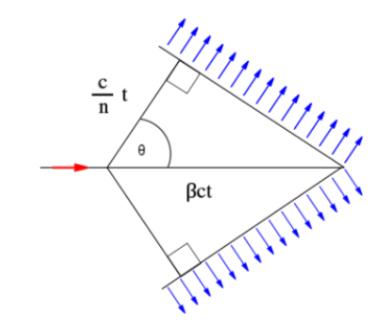
\includegraphics[width=0.3\textwidth]{graphics/Cone.png}
    \caption{Schematic representation of the Cherenkov light cone. \cite{cherenkov}}
  \end{wrapfigure}
  \FloatBarrier
The speed of light in a medium is defined by $c = \frac{c_0}{n}$, where $c_0$ is the speed of light in vacuum and $n$ the refractive index of the medium. If a charged particle travels lokally with $v_p > c$, it emits Cherenkov photons under a angle $\vartheta$. This is caused by the relaxation of the polarization of a dielectric medium. Due to the high velocity of the particle an aysymmetric polarization of the medium is created, which then leads to a Mach cone. The angle is given by
\begin{align*}
  \cos \vartheta = \frac{c/n \, t}{\beta\, c\, t} = \frac{1}{n \, \beta} \, .
\end{align*}
The cherenkov radiation has a continuously spectrum with a maximum in the UV range. The intensity is approximately proportional to the frequency of light in the visible spectrum. This is the reason why Cherenkov radiation is usually seen as blue.\\
For Cherenkov light in the atmosphere there are usually two different sources. The first cone is produced by the original particle e.g. an iron nucleus and the second one by the particle shower produced due to the original particle.
\subsection{Historical development}
P. Cherenkov discovered the light around a radioactive preparation in water in 1934. I. Tamm and I. Frank developed the corresponding the theory in 1937. All theory were awarded with the Nobel prize for their work in 1958. The first Cherenkov counter was developed in 1951 and was used to detect cosmic rays with Cherenkov light in water. A cylinder with distilled water is used as the radiator and connected to a photomultiplier. Behind it there is preamplifier to increase the signals.
Around the same time a so called getting type Cherenkov detector was designed. The radiator was a acrylic plastic cone with a top angle $\Phi$. It is followed by a lens that only focus Cherenkov light that was emitted with $\vartheta = \Phi$ trough a collimeter and is afterwards measured by a photomultiplier.
\subsection{Cherenkov detector types}
\textit{Treshold Detectors} were used in earlier collider experiments starting in 1951. They use specific mediums to distinguish differnent particles. The produced photons are beamed towards photomultipliers by using mirrors. The peak hight measured with the photomultiplier can be used to reconstruct the particle velocity. They made it possibe to distinguish between pions, kaons and protons.
\textit{Differential Cherenkov Detectors} use the angle of the Cherenkov cone together with a spherical mirror to focus the light trough a diaphragm. The radius of the diaphragm limits the measureable velocity range. Changing the preasure inside of the gas radiator controlls the refractive index. For this reason they are used to select particles instead of identifying them.\\
\textit{Ring Imaging Cherenkov Detectors} (RICH) were first designed in 1976. They can be used to reconstruct the particle speed between $0.5-\SI{150}{\giga\electronvolt}$. At higher momentums it is not possible to distinguish the Cherenkov angles of different particles. They consist of a sperical detector ($R_c$) surrounded by a mirror($R$) and the radiator is filled in between.

\begin{wrapfigure}{l}{0.5\textwidth}
    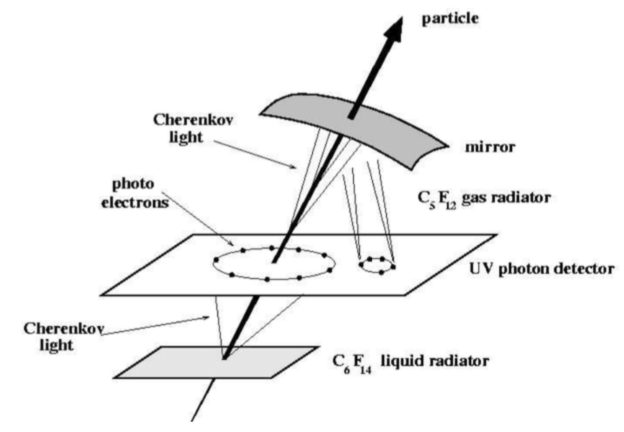
\includegraphics[width=0.48\textwidth]{graphics/RICH.png}
    \caption{RICH detector in the DELPHI experiment using two radiators and one photon detector. The Cherenkov light is projected on both sides of the detector. \cite{cherenkov}}
		\label{fig:RICH}
  \end{wrapfigure}
  \FloatBarrier

The Cherenkov light is emitted in between the detector and the mirror and reflected on the photo detector. This reflection makes it possible to calculate the velocity with $\vartheta \approx 2\frac{R_c}{R}$. Current RICH detector work with two radiators this leads to a larger momentum range as shown in figure \ref{fig:RICH}.
The main challenge for the photo detector is that it must be able to localize the spatial positio in the ring image. The Cherenkov photons are transformed into photoelectrons and measured in a multiwire propotional chamber. This leads to the reconstruction of two coordinates, the last one can be calculated from the drift time of the electrons. \textit{Detection of Internally Reflected Cherenkov light} (DIRC) is a principle where a pipe radiator is used to produce the Cherenkov light and guide it towards a light catcher. The angle information remains unchanged. This detector was used in the Babar experiment \textit{Cherenkov Calorimeter} for example made out of lead glass as a radiator. The produced light is propotional to the energy of the entering charged particles. This technology was used for the electromagnetic calorimeter of the OPAL experiment.\\
The first \textit{Imaging Atmospheric Cherenkov Telescopes}  was developed by the whipple collaboration in the early 1980. They are able to detect high gamma ray showers in a range of \SI{50}{\giga\electronvolt} to \SI{50}{\tera\electronvolt}. A large segmented, spherical mirror is used to reflect the Cherenkov light onto an array of photomultipliers. Gamma showers are usually of elliptic shape, while hadronic interactions result in broader and irregular showers due to the larger transverse momentum. Usually the Cherenkov cones cover a size of several $\SI{100}{\meter}^2$ for this reason several telescopes are grouped together to cover as much of the shower as possible. A benefit of this is, that the angular resolutions increases with each added telescope. Projection all images into one plane allows to reconstruct the originial direction of the shower. IACT detectors lead for example to the discovery of the Crab nebula in 1989. Till today they provide the best measurements of angular and energy resolution in the \si{\tera\electronvolt} domain.\\
A special use of IACT detectors are \textit{Neutrino Observatories}. The IceCUBE experiment is at the Amundsen-Scott South Pole Station in Antarctica. It consists of 86 photomultipliers that are symmetricly placed incide of a $\SI{1}{\meter}^3$ cube of ice. The ice functions as a radiator. If a neutrino reacts with the ice, it creates charged leptons that can radiate Cherenkov light. On the surface of the cube is IceTop, a detector with the purpose to detect cosmic particles and can then be used as veto for the IceCube Array. The DeepCore is build out of the 6 most inner photomultipliers, which are placed with a smaller distance. This is the reason why IceCUBE measures neutrinos in the range of \SI{100}{\giga\electronvolt} to several \si{\peta\electronvolt}. Beside the reconstruction of the energy it is also possible to determine the original direction of the neutrinos. IceCUBE measured a non-terrestrial neutrino flux in 2013. One of the most recent discoveries were the identification of two high-energy neutrino sources. Super-Kamiokande is a cylindrical water tank with a volume of around $\SI{200000}{\meter}^3$. It is placed \SI{1}{\kilo\meter} below the surface, uses the same principles as IceCUBE and the photomultipliers are positioned at the wall. Electrons produce a spheric Cherenkov ring, while the track of muons is much longer due to the slower energy loss. One of the most important discoveries of the Super-Kamiokande was the discovery of neutrino oszillation.
